\documentclass[../main.tex]{subfiles}

\begin{document}

\section{Question 6}

Model using HDL a design that can be used to implement an arithmetic right shift. Your design has to be parametric and have N-bit input, where $N \geq 4$. It should also allow to shift up to 3 positions. Do \textbf{not} use the \texttt{<<<}, \texttt{>>>} operators.

Draw a schematic of your design. Assume a value for the parameter $N = 5$.

\subsection*{Solution}

The functionality can be implemented using an array of N-to-1 multiplexers. Denoting the input and output bit-vectors $d_i$ and $d_o$ respectively, and the 2-bit select line for $s$, the circuit schematic when $N = 5$ is shown in [Figure \ref{q6}].

The output from the testbench of the implemented circuit is shown below.

\begin{mintedterminal}{Q6 - Testbench Output}
[10] Starting simulation...
[010] Input=10101010 Control=0 Output=10101010
[020] Input=10101010 Control=1 Output=01010101
[030] Input=10101010 Control=2 Output=00101010
[040] Input=10101010 Control=3 Output=00010101
\end{mintedterminal}

\begin{figure}[h]
    \centering
    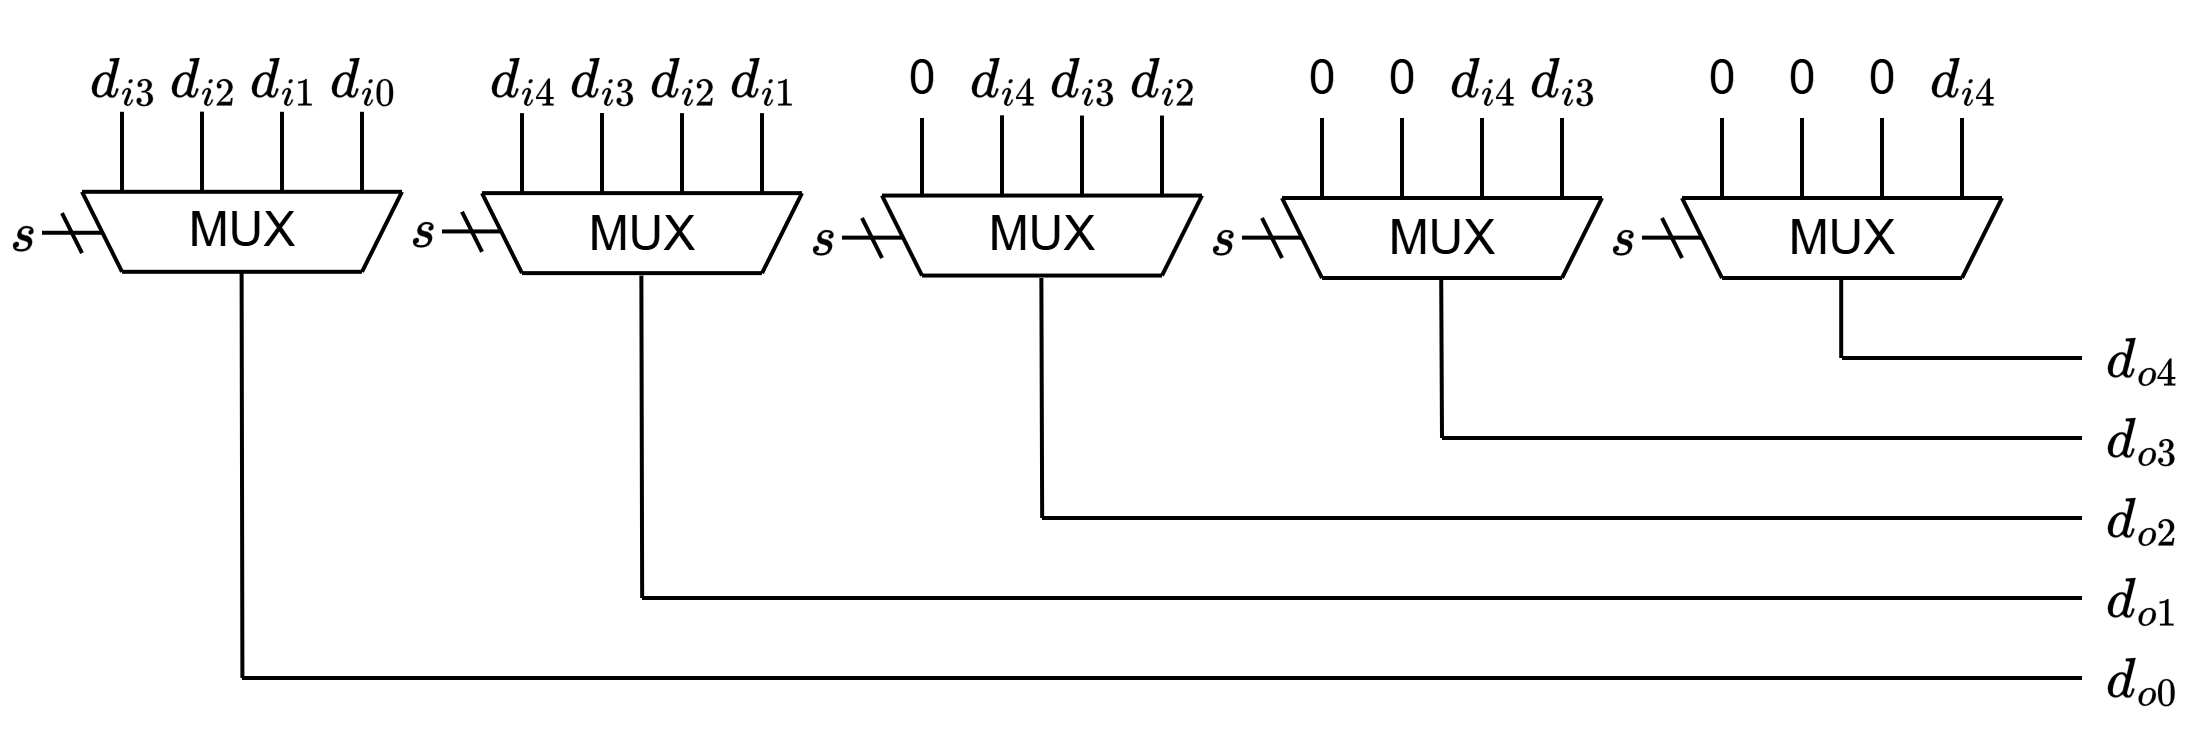
\includegraphics[width=1.0\linewidth]{assets/q6.png}
    \caption{$N = 5$ right shifter implemented using an array of multiplexers.}
    \label{q6}
\end{figure}

\newpage

\section{Question 7}

Model using HDL a signed N-bit multiplier. The design has to be parametric with 2 inputs of N-bit, where $N > 3$. Your design should use half adders and/or full adders.

Draw the schematic of your design. Assume a value for the parameter $N = 5$.

\subsection*{Solution}

To implement signed multiplication the Baugh-Wooley multiplication algorithm is used. A Baugh-Wooley multiplier is implemented as a grid of "Baugh-Wooley cells". Two types of cells are used, white and gray [Figure \ref{fig:bw_cell}]. The complete circuit diagram is seen in [Figure \ref{q7}].

The testbench iterates through all 8-bit input values and confirms the correct result is produced by the multiplier. An example snippet is shown below.

\begin{mintedterminal}{Q7 - Testbench Output}
[655270] a=127 b=118 prod=14986
[655280] a=127 b=119 prod=15113
[655290] a=127 b=120 prod=15240
[655300] a=127 b=121 prod=15367
[655310] a=127 b=122 prod=15494
[655320] a=127 b=123 prod=15621
[655330] a=127 b=124 prod=15748
[655340] a=127 b=125 prod=15875
[655350] a=127 b=126 prod=16002
[655360] a=127 b=127 prod=16129
Testbench succesfully completed!
\end{mintedterminal}

\begin{figure}[h]
    \centering
    \begin{subfigure}{.5\textwidth}
        \centering
        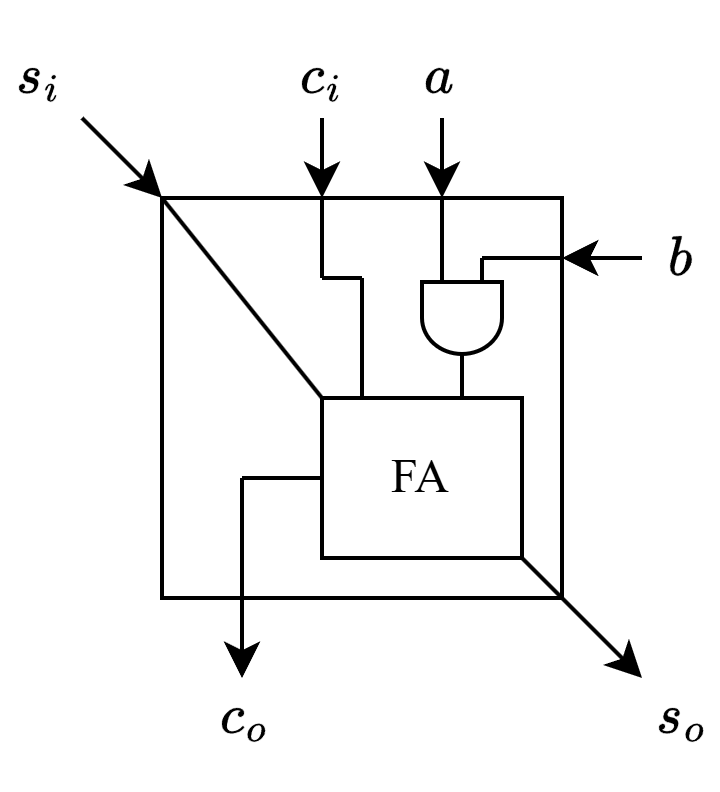
\includegraphics[width=0.8\linewidth]{assets/bw_white_cell.png}
        \vspace{-10pt}
        \caption{Baugh-Wooley multiplier white-cell.}
        \label{fig:bw_white_cell}
    \end{subfigure}%
    \begin{subfigure}{.5\textwidth}
        \centering
        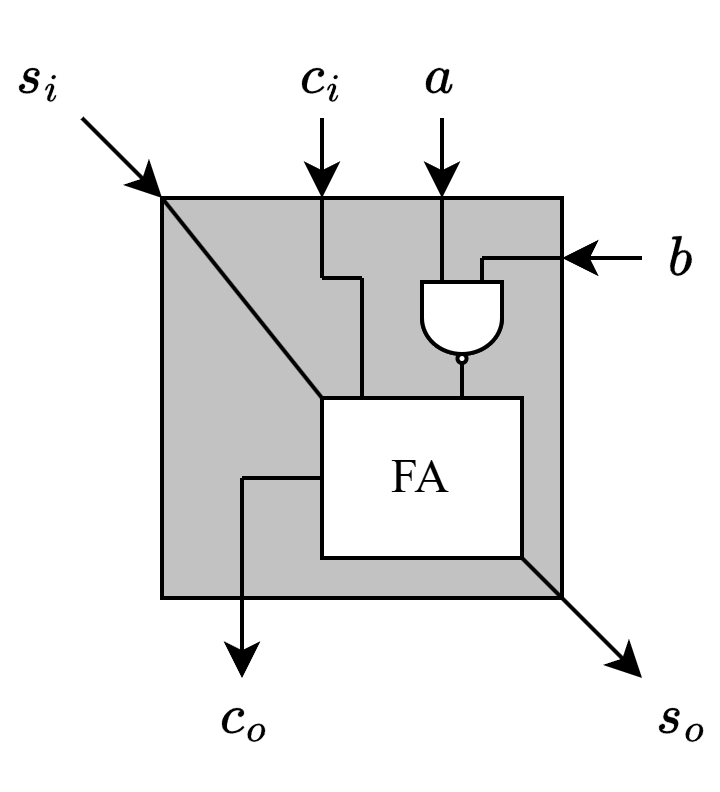
\includegraphics[width=0.8\linewidth]{assets/bw_gray_cell.png}
        \vspace{-10pt}
        \caption{Baugh-Wooley multiplier gray-cell.}
        \label{fig:bw_gray_cell}
    \end{subfigure}
    \vspace{-10pt}
    \caption{Baugh-Wooley multiplier basic cell construction.}
    \label{fig:bw_cell}
\end{figure}

\newpage

\begin{figure}[H]
    \centering
    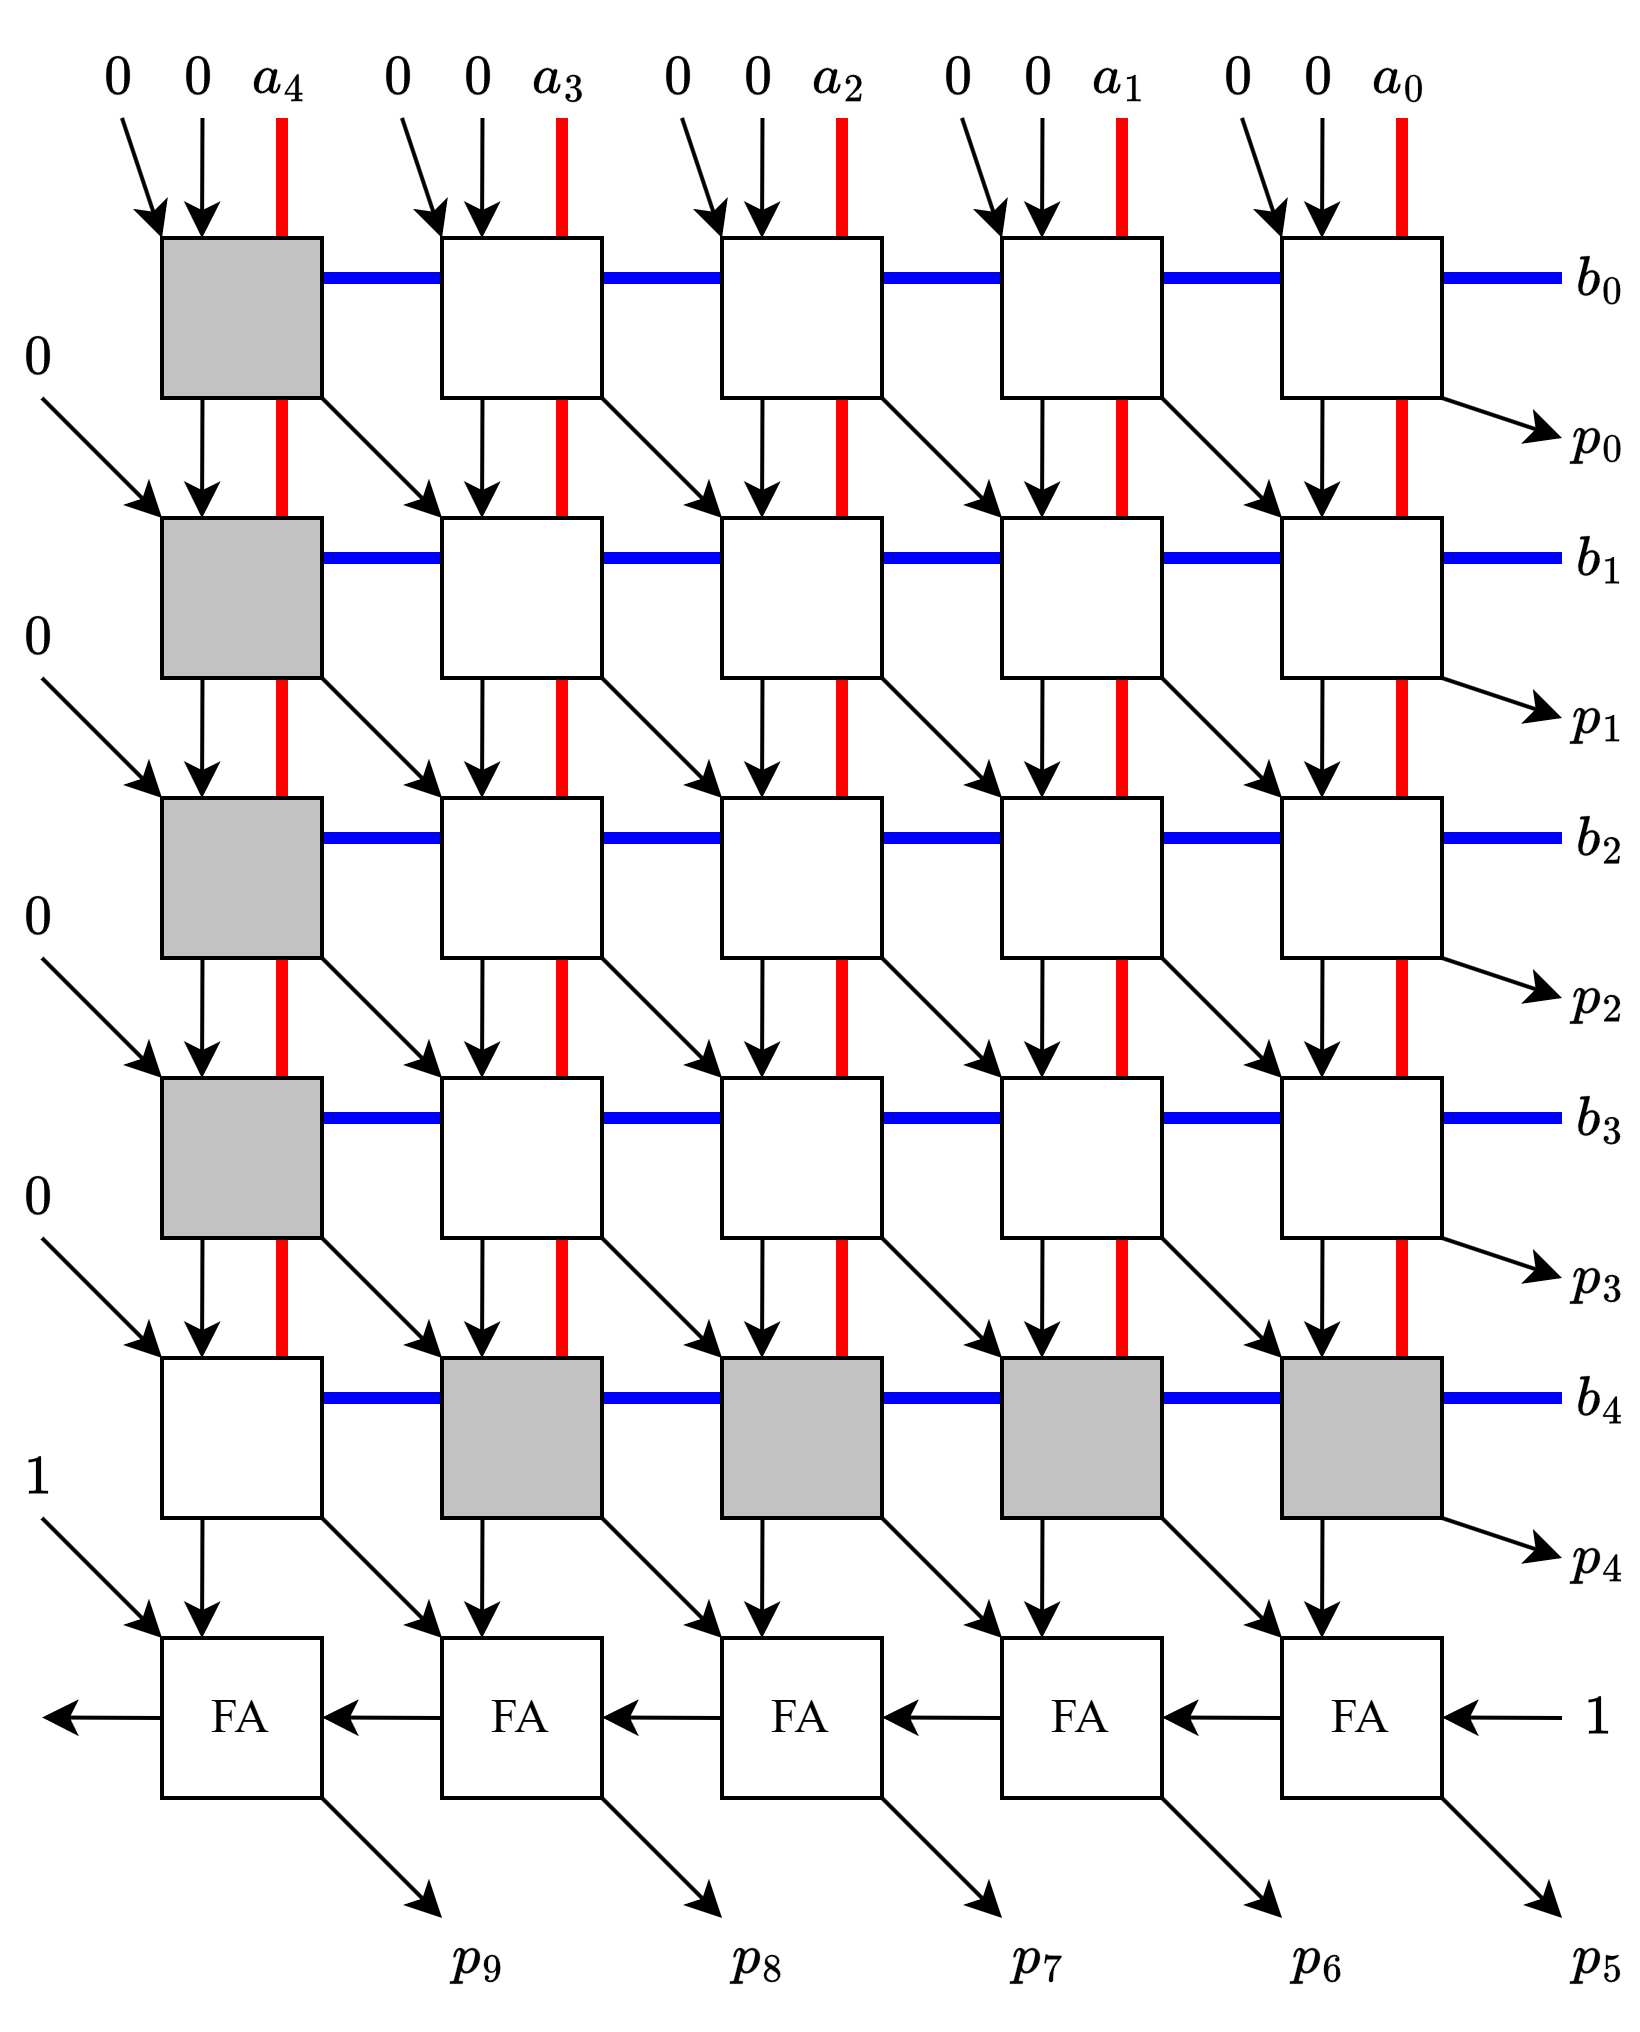
\includegraphics[width=1.0\linewidth]{assets/bw_5bit_multiplier.png}
    \caption{Block diagram of a $N = 5$ Baugh-Wooley multiplier implemented using basic Baugh-Wooley white- and gray-cells. Inputs are denoted $a$, $b$, and the product is denoted $p$.}
    \label{q7}
\end{figure}

\newpage

\section{Question 8}

Model using HDL a design that can multiply 6 N-bit numbers and add the results. The design should be parametric with parameter N. You must ensure that your design does not overflow or underflow and assign the correct bit width for all intermediate and output signals. The design should implement the following equation:

$$
    \text{out} = \sum_{k \in {0, 2, 4}} X_k \cdot X_{k + 1}
$$

Draw a schematic of your design. Assume a value for the $N = $ parameter.

\subsection*{Solution}

The module is implemented using the previous Baugh-Wooley multiplier and multiple carry-lookahead adders. The schematic is shown in [Figure \ref{q8}] and the testbench output is shown below.

\begin{mintedterminal}{Q7 - Testbench Output}
[010] a=0 b=0 c=0 d=0 e=0 f=0 res=0 expected=0
[020] a=1 b=2 c=3 d=4 e=5 f=6 res=44 expected=44
[030] a=10 b=20 c=5 d=8 e=100 f=2 res=440 expected=440
[040] a=-1 b=10 c=-5 d=4 e=1 f=-1 res=-31 expected=-31
[050] a=127 b=127 c=127 d=127 e=127 f=127 res=48387 expected=48387
[060] a=-128 b=-128 c=-128 d=-128 e=-128 f=-128 res=49152 expected=49152
\end{mintedterminal}

\begin{figure}[h]
    \centering
    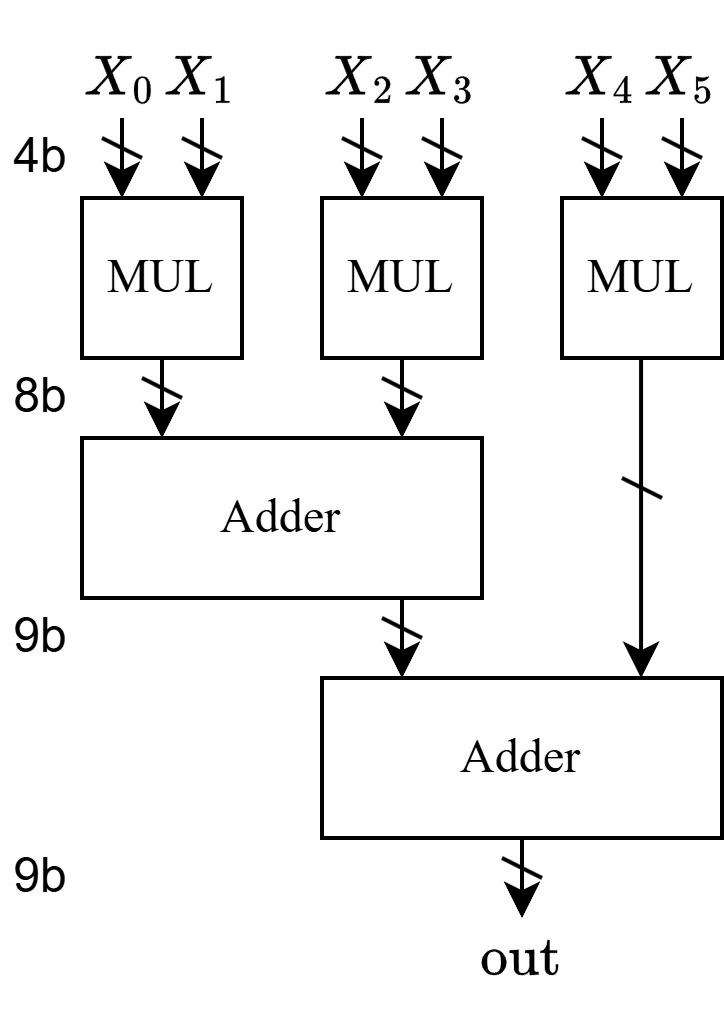
\includegraphics[width=0.4\linewidth]{assets/q8.png}
    \caption{Block diagram of the 6 number multiply/accumulate module with $N = $.}
    \label{q8}
\end{figure}

\newpage

\section{Question 9}

Model using HDL an unsigned multiplier that can be used to multiply two 16-bit numbers. The multiplier should be built usnig components of multiple 4-bit multipliers. The 4-bit multiplier can be modelled behaviorally by using the (*) operator.

Draw a schematic of your design.

\subsection*{Solution}

We first construct a 8-bit multiplier from four 4-bit multipliers and three 16-bit adders as shown in [Figure \ref{q9_1}]. Denoting the 8-bit inputs $a$, $b$, they are split into 4-bit halves $a_L, a_H, b_L, b_H$. The halves are fed into the 4-bit multipliers and their products are bit-shifted and added to produce the final 16-bit product. The same approach is taken to create the 16-bit multiplier, but instead of using behaviorally modelled 4-bit multipliers and 16-bit adders, it uses the 8-bit multiplier from [Figure \ref{q9_1}] and 32-bit adders. The block diagram is shown in [Figure \ref{q9_2}].

\begin{figure}[h]
    \centering
    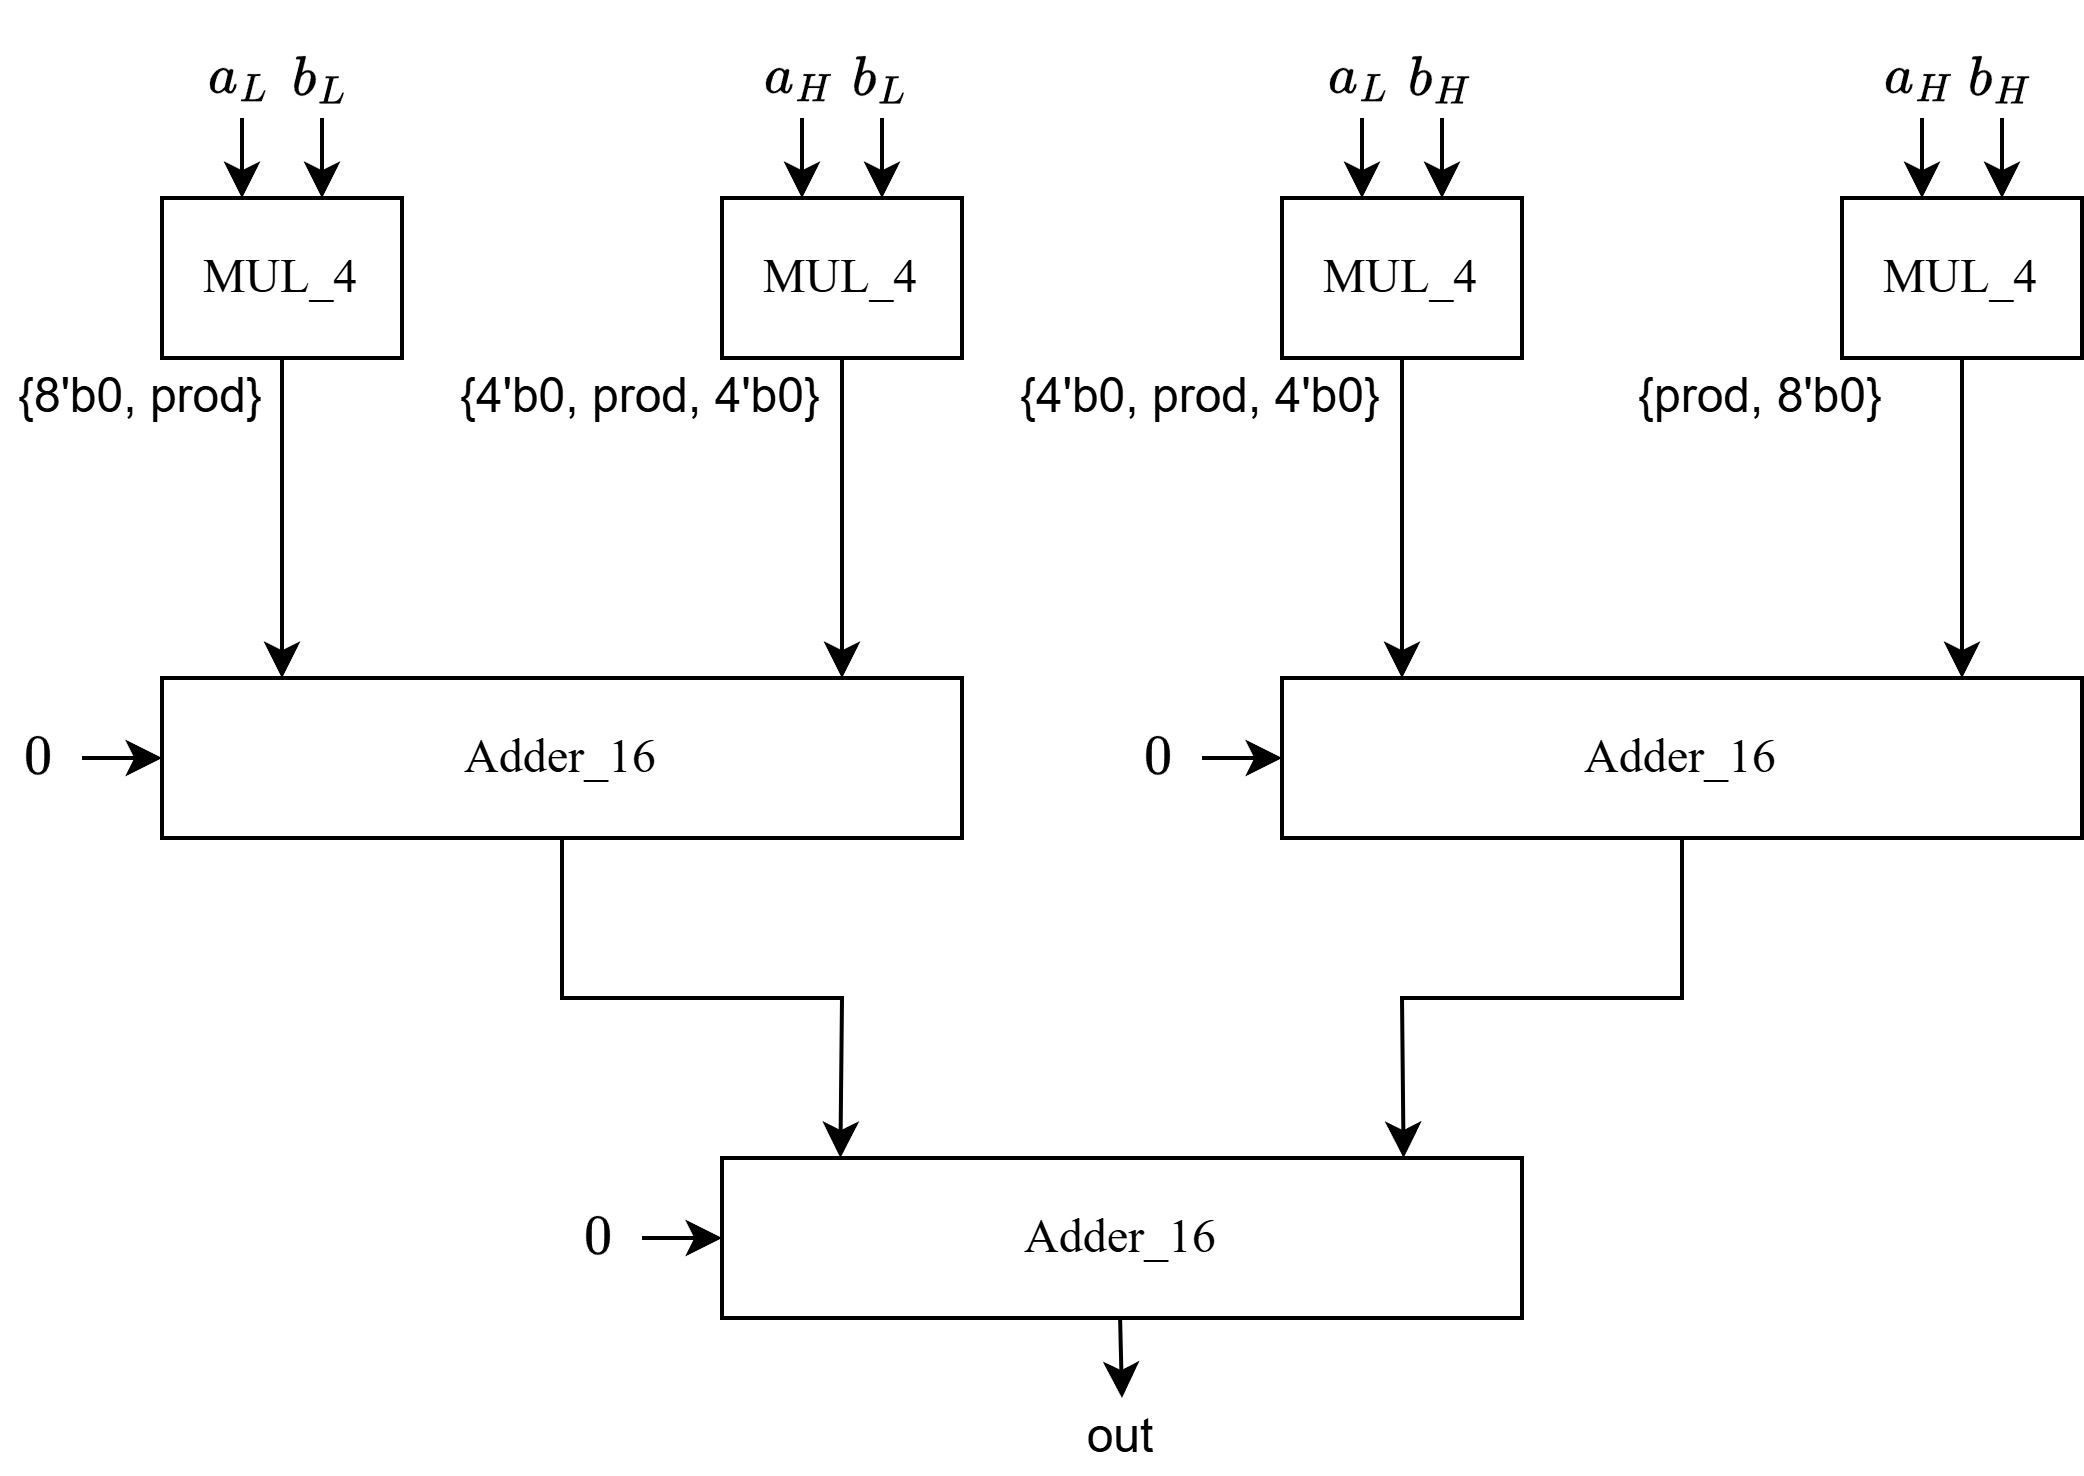
\includegraphics[width=0.6\linewidth]{assets/mul_8.png}
    \caption{Block diagram of 8-bit multiplier made from 4-bit multiplier and 16-bit adder modules.}
    \label{q9_1}
\end{figure}

\begin{figure}[h]
    \centering
    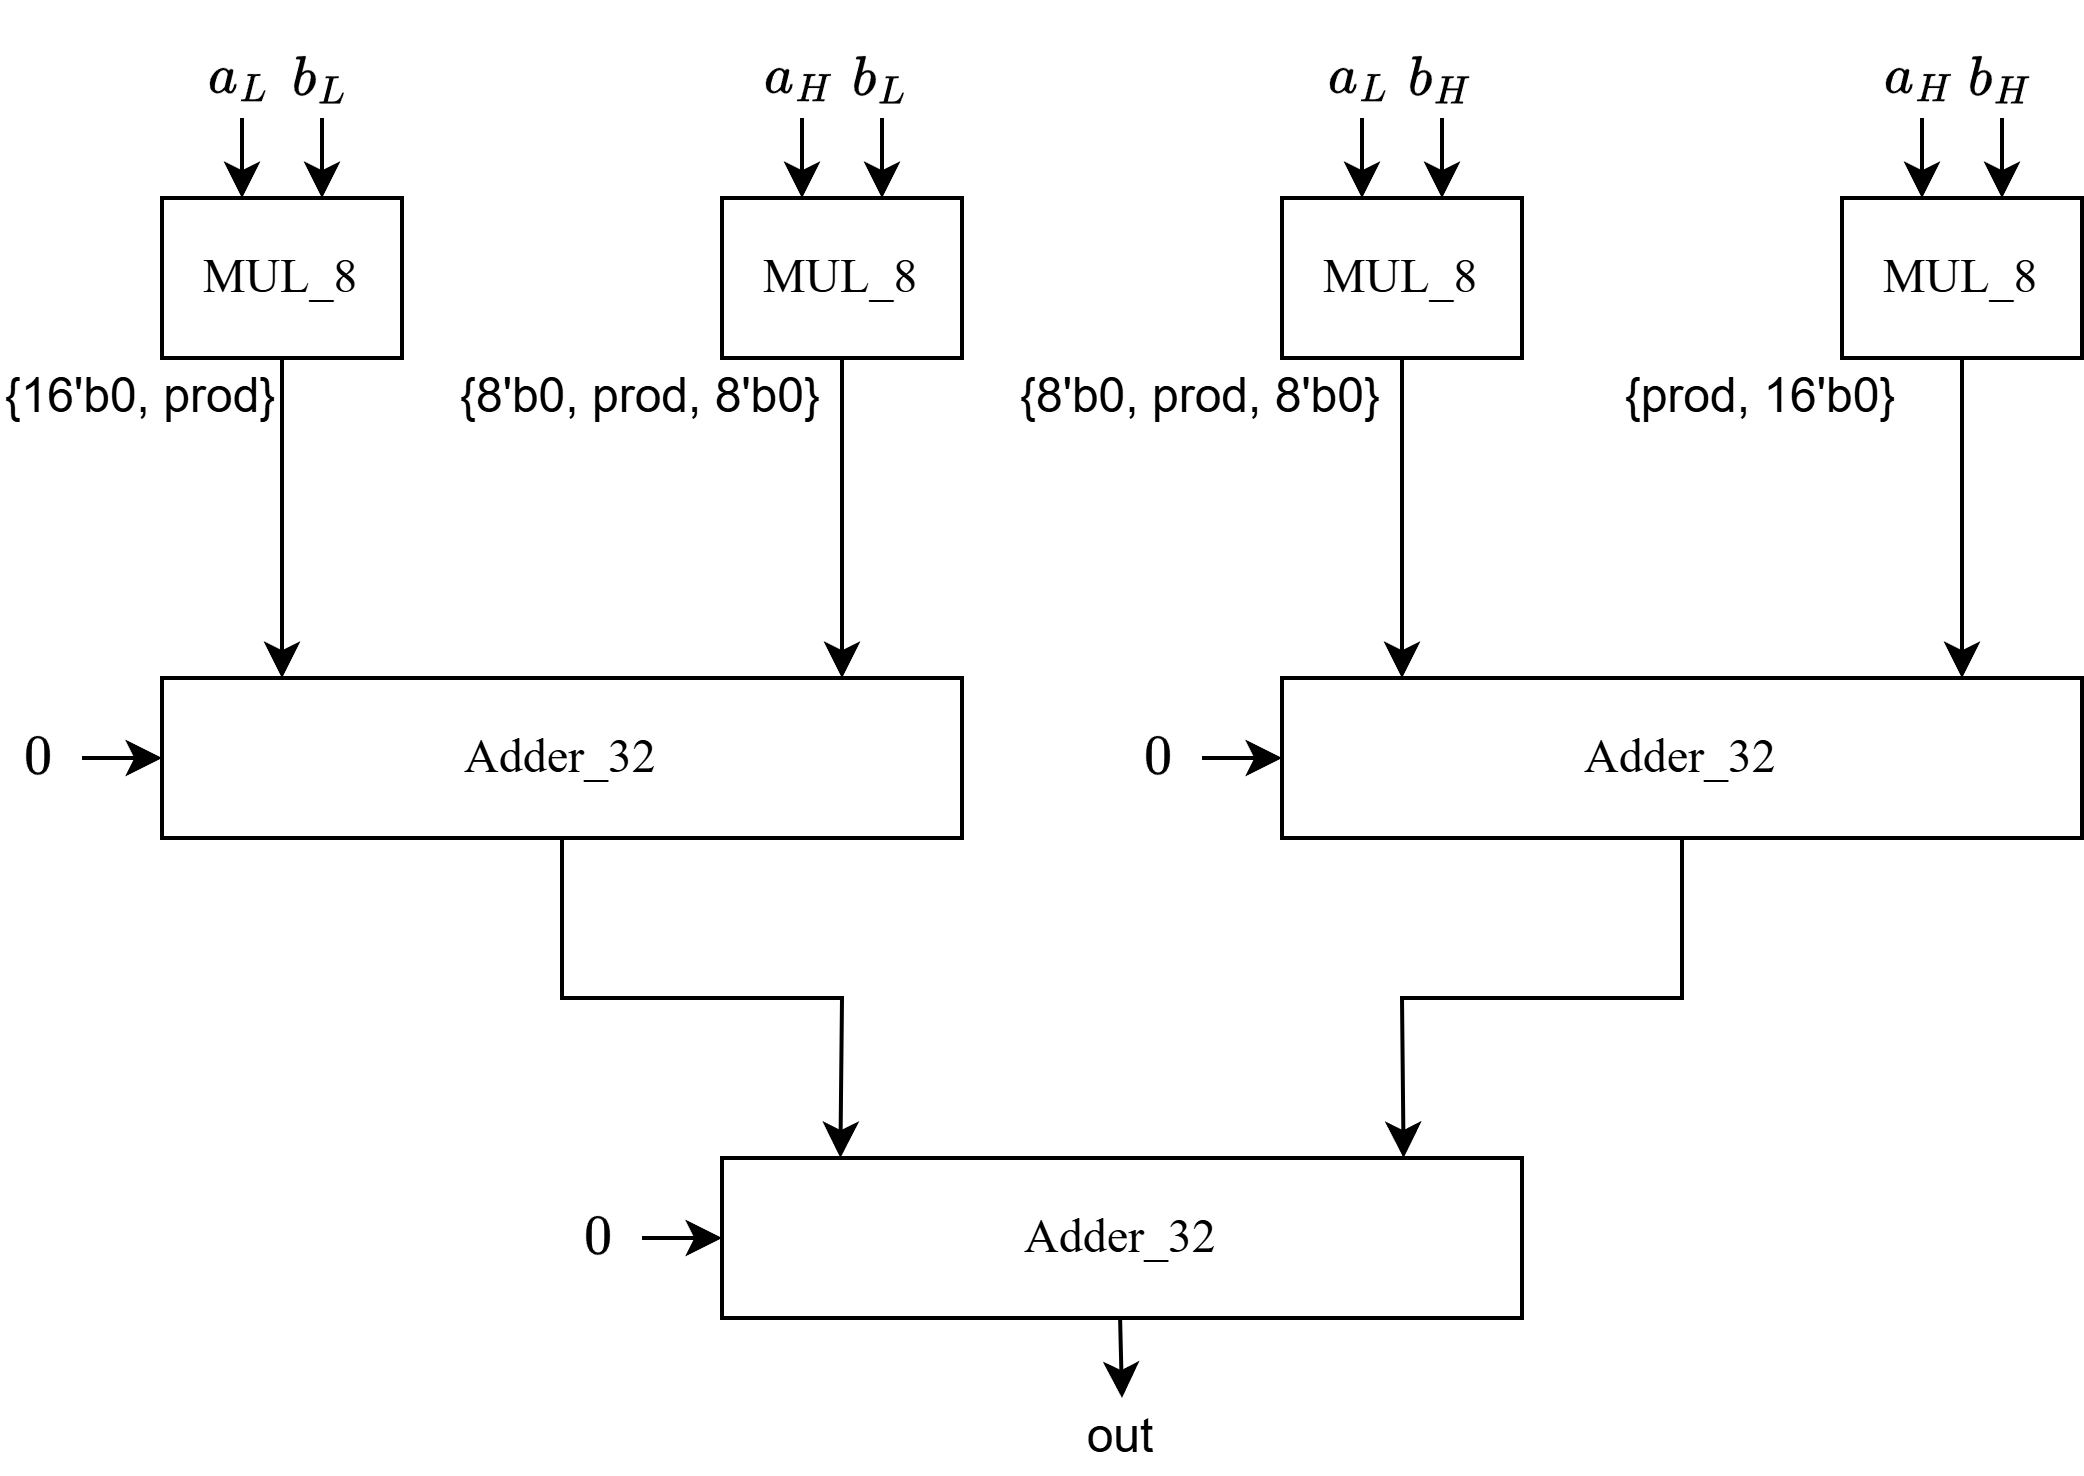
\includegraphics[width=0.6\linewidth]{assets/mul_16.png}
    \caption{Block diagram of 16-bit multiplier made from 8-bit multiplier and 32-bit adder modules.}
    \label{q9_2}
\end{figure}

\end{document}
